% -*- coding: utf-8 -*-

\chapter{Planificación. Diagrama de Gantt}\label{gantt}

En la figura \ref{fg:gantt} se muestra el diagrama de Gantt de la planificación del proyecto. El desarrollo del mismo ha tenido una duración de casi 20 meses, incluyendo la fase inicial de formación. El comienzo tuvo lugar en marzo de 2006 y la finalización se establece a mediados de octubre de 2007.

La mayor parte de la etapa de formación previa (actividades 1, 2 y 3) abarca desde marzo de 2006 hasta octubre de 2006, aunque alguna de sus subtareas se llevaron a cabo fuera de este periodo de tiempo. La familiarización con el robot Urbano (actividad 3 del diagrama) tuvo varias fases. La primera se desarrolló en septiembre de 2006 y fue una primera puesta en contacto con el robot para conocer su funcionamiento básico y parte de la base de navegación disponible. En mayo de 2007 se comenzó a trabajar con las clases ya existentes descritas en el capítulo \ref{ch:arquitectura}. En septiembre de 2007 se realizó la mayor parte de las pruebas con el robot y se emplearon distintas formas de conexión con el mismo.

Una vez se hubo implementado el regulador para llevar a Urbano de un punto a otro (actividad 9), se definieron las trayectorias para que el robot recorriera sus puntos secuencialmente (actividad 11). Posteriormente se centró el trabajo en el regulador de acercamiento a una trayectoria definida (actividad 12) y, a continuación, en la forma de suavizar dicha trayectoria (actividad 13). Cuando se trató de implementar un sistema análogo en el robot P3AT surgieron algunas dificultades. Se comenzó por consultar los manuales del robot así como la documentación y ejemplos de la librería Aria (actividad 4) para ir desarrollando algunos programas iniciales (actividad 5). En algunos casos el comportamiento no era el esperado, debido a que Aria requiere versiones de Visual Studio posteriores a la versión 7. Esto desemboca en el paso a la versión 8, Visual.Net 2005, para lo que fue necesario reinstalar y recompilar las librerías en varios modos y en varios PCs y comprobar que los errores ya no se producían (actividad 6). Una vez estuvo todo correcto, se pudo hacer uso del sistema para el P3AT, después de modificar el controlador (actividad 10). Paralelamente se iba estudiando el estado del arte relativo a planificación de trayectorias y control reactivo (actividad 8, previamente se había estudiado teoría sobre \emph{motion control} y cinemática de robots). Finalmente, se implementó el algoritmo de deformación de trayectorias para evitar los obstáculos (actividad 14). Simultáneamente a la construcción de estas componentes del sistema se iban realizando pruebas que garantizaran su buen funcionamiento (actividad 25) La mejora de la interfaz de usuario (actividad 16) se llevaba a cabo según iba resultando conveniente. La última actividad dentro del marco de control de movimiento, planificación de trayectorias y control reactivo (actividad 7) fue la introducción de nuevas acciones de control (actividad 15), medida tomada a la vista de los resultados obtenidos con el robot real.

A finales de marzo de 2007 empezó el trabajo sobre localización y mapas (actividad 17). En primer lugar fue necesario el estudio del estado del arte (actividad 18). Cuando se hubo completado éste, se efectuó la implantación del algoritmo escogido para la localización del robot y la elaboración de mapas (actividad 19). Al mismo tiempo se iban realizando experimentos y pruebas (actividad 26), y se vio la conveniencia de reducir el tiempo de procesamiento que consumía la ejecución de dicho algoritmo (actividad 20). Posteriormente se introdujeron nuevos botones en el diálogo para poder guardar y leer mapas y datos de ficheros, para poder inyectar ruido, para poder seleccionar la estimación del ruido de la odometría que ha de utilizar el filtro...(actividad 22). Una última actividad de este apartado fue la selección e implementación del algoritmo para borrar puntos dinámicos del mapa (actividad 21).

La integración de las dos partes diferenciadas del sistema (actividad 23) se realizó cuando estuvieron prácticamente finalizadas ambas.

Los experimentos y pruebas finales con el robot real (actividad 27) se desarrollaron a finales de julio de 2007 y durante septiembre/ principios de octubre, del mismo año.

La documentación del proyecto (actividad 28) abarca desde principios de julio hasta mediados de octubre de 2007.

\clearpage
\begin{figure}
  % Requires \usepackage{graphicx}
  \centering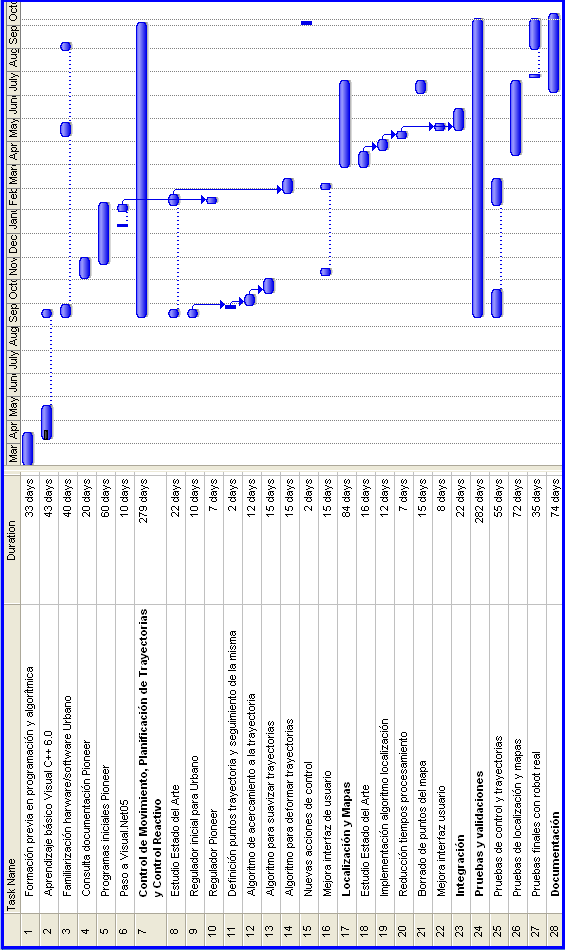
\includegraphics[scale=0.6]{gantt6}\\
  \caption{Diagrama de Gantt}\label{fg:gantt}
\end{figure}
